\section{connectivity}
In the following section I will discuss how the classification will be presented to the user.

\paragraph{Overview}
As previously outlined in the design section, I would like for the information to be displayed as a webpage hosted on the Pi. This will
require several components:
\begin{itemize}
    \item Web page: for the actual displaying of information
    \item API: for the sending and receiving of the information form the AI model to the user
    \item WIFI Hosting: to allow the user to connect to the device in a dynamic setting rather than using a common network which may or
    may not exist in a movable setting such as a car

\end{itemize}

\subsection{Back-End:}
\paragraph{Network Architecture and Hosting}
By utilizing Raspberry Pi OS (Desktop), I can easily toggle between “Hotspot Mode” for device testing and “WI-FI Client Mode” for pulling
updates via Git. This flexibility of duel purpose drastically accelerated the development and testing cycle of this section of the project,
with the ease of not needing to type commands or form a toggle file.
\paragraph{Initial Flask Implementation}
To validate the connection, I developed a light-weight Flask application to serve a basic index.html file. This contained no information,
images or other resources, just text. This confirmed that devices could successfully connect to the Pi’s hotspot and access the web
server by inputting the Pi’s IP address.
This application was constructed to specifically use port 80 (HTTP), removing the need to define the connection protocols when handling
IP addresses (Such as when changing the hostname)
\paragraph{Local DNS Resolution}
To provide a seamless user experience, I wanted to remove the IP-based navigation and instead navigate with a custom hostname. To do this
I used ‘dnsmasq’. Using this, I configured the domain “drowsiness” directly to the local IP address for the application.
\paragraph{Performance Optimisers (DNS Upstream)}
Since the system operates as an offline connection, with no external internet access, I disabled recursive DNS lookups\footnote{the
process where a device tries to ask other (more senior) servers for corresponding IP addresses for addresses outside of its local
scope/knowledge}.
This improves the performance by preventing the Pi from attempting to contact upstream servers for un-known queries, eliminating the
latency caused by waiting for timeout responses.
However, with this in mind, it is important that this change is reverted when connecting to the wider internet as this can prevent you
from accessing resources such as the GitHub repository. To revert simply remove “no-resolv” from /etc/dnsmasq.conf. \TODO{remmeber this}


% dnsmasq code section
\begin{minipage}{\textwidth} % ensures it is not split across pages
    \begin{mdframed}[style=takeawaybox]
        \begin{lstlisting}[language=bash, caption={dnsmasq Configuration}, captionpos=b]
            no-resolv
            no-poll
            interface=wlan0
            address=/drowsiness/10.42.0.1
            dhcp-range=10.42.0.2,10.42.0.254,255.255.255.0,24h
            dhcp-option=3,10.42.0.1
            dhcp-option=6,10.42.0.1
            # Configuration file for dnsmasq.
        \end{lstlisting}
    \end{mdframed}
\end{minipage}

% Explanation box for each line
\begin{table}[H]
\centering
\caption{Explanation of dnsmasq Configuration Parameters}
\label{tab:dnsmasq_explained}
\begin{tabularx}{\textwidth}{|l|X|}
\hline
\textbf{Configuration Line} & \textbf{Functional Explanation} \\ \hline
\texttt{no-resolv} & Tells the system not to look at the system's \texttt{/etc/resolv.conf} file, preventing it from using the ISP's
upstream DNS servers. \\ \hline
\texttt{no-poll} & Stops the service from checking for changes in the upstream DNS configuration files. While not strictly necessary,
it helps maintain system cleanliness. \\ \hline
\texttt{interface=wlan0} & Restricts the service to listen only for requests on the Wi-Fi interface. This allows the Ethernet connection
to remain independent for interacting with the GitHub repository. \\ \hline
\texttt{address=/drowsiness/10.42.0.1} & Acts as a local DNS redirect for the 'drowsiness' domain, pointing it directly to the
application's IP. \\ \hline
\texttt{dhcp-range=...,24h} & Defines the pool of valid IP addresses a connecting device can be assigned. This lease lasts for 24 hours. \\
\hline
\texttt{dhcp-option=3,10.42.0.1} & \textbf{Option 3 (Default Gateway):} Tells connected devices to send their internet-bound traffic to
this machine (10.42.0.1). \\ \hline
\texttt{dhcp-option=6,10.42.0.1} & \textbf{Option 6 (DNS Server):} Instructs connected devices to use 10.42.0.1 as their primary DNS
server. \\ \hline
\end{tabularx}
\end{table}

\paragraph{Multi-User Scalability}
To allow for multiple devices to connect at once, I configured a /24 subnet mask to manage IP assignments. While the Raspberry Pi’s hardware typically supports 5-10 devices connected concurrently, this ensures that:
\begin{itemize}
    \item Multiple passengers can connect without causing IP conflicts
    \item The driver’s connection remains stable, ensuring that safety critical data is always accessible, even if other devices accidently “auto-join” the network
\end{itemize}

\begin{figure}[H]
    \centering
    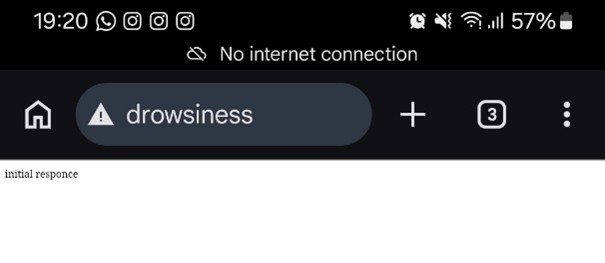
\includegraphics[width=0.6\textwidth]{Images/blankWebpage.jpg}
    \caption{This is a Simple example of how a webpage URL can be inputted to make it easier for the user to find the resource. In this example, while ‘drowsiness’ worked on one browser,  ‘drowsiness/’ had to be used on another as it assumes it is a search not a URL.}
\end{figure}

\paragraph{Captive Portal}
One of the other features that would be ideal is the use of a Captive Portal. Often, when connecting to public or guest Wi-Fi networks
(such as a coffee shop or cinema) you must go through a page to accept their terms of conditions and potentially log-in. While I will
not be using a log-in system, agreeing to terms and notifying the user of issues using the phone may cause would be a good moral stead,
as well as it then easily allowing the user to interface/view the webpage after acknowledging the potential risk.
This will be done by using DNS hijacking.
\TODO{more about this}

\paragraph{API}
As previously mentioned, I have opted for an integrated API and AI model solution, where the model work to use in-memory state management rather than a database or file; the main reasons being to reduce complexity by avoiding I/O overhead provided from databases
and avoid race conditions.

\paragraph{Structure}
The API file will be broken into 3 sections for simplicity and ease of use:
\begin{itemize}
    \item\textbf{Flask Initialization}
        Since this file will eventually be run on start-up of the device, rather than a manual start up (so that the system is up
        and functional for ease of use), I have decided to group the initialization of the webpage to this file. While this could
        be separated out, the simplistic nature allows for a cheap and easy way of ensuring everything is functional. Additionally,
        with it being an operation which calls other processes, it also allows for other areas of the project to load in the mean-time
        (e.g. load the AI model from memory).
        Furthermore, this asynchronous initialization… \TODO{finish}
    \item\textbf{Prediction Generation}
        This will allow for both the model’s predictions and the calling function to have access to the same variables. By using
        threading, I can continuously run the model without interfering with other procedure calls, allowing for seamless and continual
        integration. This is especially important when considering the multi-user capabilities. If the webpages are not synced (highly
        likely), API calls from each independent version of the webpage would otherwise cause the AI model to stop capturing data while
        the calls are answered. This would result in fewer frames being captured and processed, increasing latency to this critical safety
        system.
        While the use of threading can invoke race conditions by each thread trying to both interact with the same variable,
        ‘thread.Lock()’ is used to freeze a variable during assignment or reading to only allow one process to use this variable at a
        time.
    \item\textbf{Web Call Processing}
        Rather than refer to a direct IP address (which may vairy between devices and can be dependent on other connections), this API
        call uses relative URL routing to easily find the correct API. This is potentially less secure, however, with the final aim being
        to remove all other processes and files and only have the API, webpage and AI model on the device, here is little more that a
        potential attacker could do. 
        In an ideal world, with the correct hardware which is tailored specifically to this project, forming a more market focused product,
        the scope of what could be done would be reduced and \TODO{finish this off}
\end{itemize}


\subsection{Front-End:}
\paragraph{Webpage Design}
The primary objective of the front-end interface is to communicate the user’s predicted alertness efficiently while maintaining a
discrete aesthetic. To ensure the interface is non-intrusive during general use – regardless of ambient lighting – a permanent dark-mode
theme will be implemented. This will minimize user distraction and reduce eye strain during both day and night time use. 
\paragraph{Design Ideas}
This section will give some examples of potential ideas. Some of these ideas will not make it into the final product, but may wish to be
considered in other related projects or in the event this project is done again.
\TODO{insert sketches and ideas}
\TODO{end with one idea as a final choice and explain each idea and its pro/cons}
\paragraph{Integration}
Following the construction of a basic frontend, I wanted to see how it would look as a changing display – using random variable
generation to get a better view of the system. To do this, I simply used the ‘random’ function to generate appropriate (possible)
values and store them in the shared variables to be sent upon API call.
\TODO{Insert Image}
\begin{figure}[H]
    \centering
    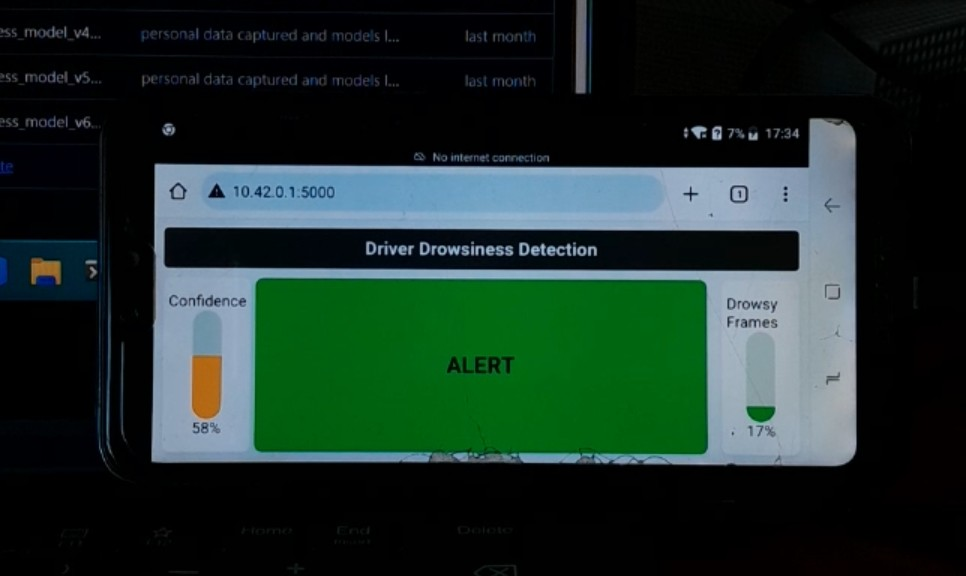
\includegraphics[width=0.6\textwidth]{Images/basic_integrated_webpage.jpg}
    \caption{Example of a simple webpage layout.}
\end{figure}